\documentclass[twoside]{article}
\usepackage[utf8]{inputenc}
%\usepackage[uebung, answers]{tumbgdm}
\usepackage[klausur]{tumbgdm}
\usepackage{lecturesetup}
\usepackage{pdfpages}
%\nummerUebungsblatt{6}
%\nummerErsteFrage{14}
\klausurTitle{Exam Computational Foundations I \\(LRG0060, WS 2021/22)}
%\LearningOutcome{
%We are warming up with C/C++ programming environments.
%}
\lstset{numbers=left, stepnumber=1}
\begin{document}

\maketitle
% 90 points for 90 minutes
\evaluationtable

\clearpage

\begin{task}{Multiple Choice}{5}{}
  Answer the following questions with yes or no. \\
  \emph{A wrong answer is counted as -1, a correct answer is counted as +1, an answer not given is counted as 0 (if you don't know the answer it is smarter not to give an answer!). If you reach more than 5 points, the points will become bonus points, if you reach less than 0 points, the result is 0 points.}
  \vspace{2cm}
  
\begin{mclist}
  \mcquestion{In MATLAB, subsets of data can be created with slicing.}{X}{}{}
 \mcquestion{In MATLAB, one needs to allocate memory for an object before creating or using it using malloc and free.}{}{X}{}
 \mcquestion{For arbitrary large $n$, an algorithm of runtime complexity $O(n)$ will become faster than an algorithm of $O(n^2)$.}{X}{}{Of course}
 \mcquestion{The SDL libraries are a collection of linear algebra routines such that we can easily solve numeric problems in C++.}{}{X}{SDL = Simple Direct Media Layer = simple GUI framework.}
 \mcquestion{MATLAB is a compiled language generating native executables.}{}{X}{}
 \mcquestion{C++ is a compiled language generating native executables.}{X}{}{}
 \mcquestion{A complete binary tree with depth $n$ has $2^n$ leaf nodes.}{X}{}{}
  \end{mclist}

   


\end{task}
\clearpage
\begin{task}{Algorithm Representation}{5}{}
  Consider the Algorithm in Listing \ref{lst:listing1}
  \begin{lstlisting}[caption=An imperative program, label=lst:listing1]
    DECLARE A,B,C,D,E,RESULT
    A = 1;
    B = SQUARE(A);
    C = 3;
    D = 4;
    E = C+D;
    RESULT = E*B;
\end{lstlisting}

  \begin{enumerate}
  \item {Write a table with a row for each line of the previous program and a column for each variable declared and give the value \textbf{after} the line has completed. Use a ? if the value is unknown (e.g., the variable has not yet been initialized). Include Line 1 (which just means every variable value is unknown).
    \vspace*{8cm}}
    \clearpage
    
  \item{Consider the following program:
\begin{lstlisting}
A = CIRCLE(P, R);
B = CIRCLE(Q, R);
M1, M2 = INTERSECT(A,B);
L = LINE(M1,M2)
RESULT = INTERSECT(L, LINE(P,Q))
\end{lstlisting}


    Give the same program as a single expression for result. That is, not using multiple lines of imperative code, but braces to organize the computation of the result.
    \vspace*{4cm}}

  \item{Assume P, Q are given points, R is the radius of the circles and the length of the segment from P to Q, INTERSECT returns two intersection points of geometries (either of two circles or of two lines), LINE constructs a line between two points. Draw what the program does. Give variable names as labels for the objects you draw.\vspace*{2cm}}

    
  \end{enumerate}
  
  
\end{task}
\clearpage

\begin{task}{Turtle Graphics}{5}{}
  Consider a turtle with commands \code{m} for move, \code{l} for turn left by $90^\circ$ and \code{r} for turning right. The turtle starts in the marked position.
  
  \centering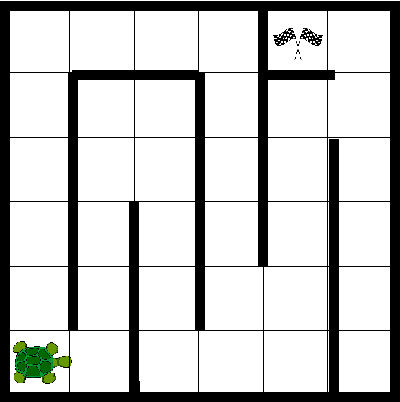
\includegraphics[width=.4\textwidth]{gfx/turtlemaze.pdf}

  \begin{enumerate}
  \item{Sketch an imperative program that gets the turtle into the goal location not crossing bold walls. Denote the program as a string consisting of aforementioned characeters. For example \code{ml} means move and then turn left.\vspace{2cm}}
  \item{
    Now, we add a simple sensor to our turtle: It is always able to check whether it can move forward by running a
    C++ function \code{bool empty()}. In this context, the movement commands are implemented as C++ function \code{move()}, \code{turnleft()}, and \code{turnright()}. Give a short C++ program (without any function declaration, just the functional body) that solves the maze using \code{while} loops to avoid repetitions of commands. Write up to three columns - the program is not short.
  }

  \end{enumerate}


\end{task}
\clearpage

\begin{task}{Bubble Sort}{15}{}
  Consider the C++ program in Listing \ref{lst:bubblesort}. The function print just outputs a space-separated list of the values of the argument vector and its implementation details can be ignored. 
  \lstinputlisting[caption=Bubble Sort, label=lst:bubblesort]{code/bubblesort.cpp}

  \begin{enumerate}
  \item{How often is the inner loop (L17-L22) executed?\vspace{2cm}}\clearpage
  \item{Create a table with the state after execution of Line 21 by reporting n, i, and the entries of A. Give the first 8 lines of this table only.\vspace{12cm}}
  \item{Define the term ``Loop Invariant'' in one sentence. Only the first given sentence is taken into account. \vspace{3cm}}
    \end{enumerate}
\end{task} % Give implementation, let students run it
\clearpage

\begin{task}{Turing Machine}{10}{}
  Given a Turing machine with a finite string of 0s and 1s on the tape, delimited in both directions with empties $\epsilon$,
  implement an algorithm that detects an instance of a three consecutive ones. Implement the Turing machine with states
  \code{start} for the beginning, \code{found} for the case that a triple one  was found, and \code{notfound} otherwise. The band can be in arbitrary states afterwards. We only consider the final state as relevant.

  \begin{enumerate}
  \item{Give the machine as a transition table. The table can be incomplete. As agreed, the machine will halt if there is no applicable rule. \vspace{10cm}}
  \item{Which of the following properties do Turing machines have? Answer yes or no:
    \begin{itemize}
    \item {they are deterministic: \vspace{1cm}}
    \item {they are not determined:\vspace{1cm}}
    \item {they are capable of computing the sum of numbers:\vspace{1cm}} 
    \end{itemize}
      }
  \end{enumerate}

  
% for turingmachine.io
%input: '000100101011011100101010'
%blank: ' '
%start state: start
%table:
%  start:
%    1: {R: state_once}
%    0: {R: start}
%    ' '  : {R: notfound}
%  state_once:
%    1: {R: state_twice}
%    0: {R: start}
%    ' '  : {R: notfound}
%  state_twice:
%    1: {R: found}
%    0: {R: start}
%    ' '  : {R: notfound}
%  found:
%  notfound:
  \end{task}
  \clearpage
  
  \begin{task}{Markov Algorithms}{10}{}
    Markov algorithms have been introduced to simplify the analysis and implementation of Semi Thue Systems. \emph{Note: This task illustrates, that Markov algorithms are Turing complete in that we give an example of an encoding of a Turing machine as a Markov algorithm.}

    \begin{lstlisting}[caption=Implementing a Turing machine as a Markov Algorithm]
S0 -> R0
R0 -> 0R      
R1 -> 1R
R  -> C
1C -> C0
0C -> 1X
0X -> X0
1X -> X1
X -> H 
      \end{lstlisting}
    
    \begin{enumerate}
    \item {What is the key difference (1 sentence) between Semi Thue systems and Markov algorithms?\vspace{2cm}}
    \item{Execute the given Markov algorithm on the input strings ``S001'' and ``S010''. Give all intermediate strings and (preferably for correction) the line number of the rule you applied. Tip: Write your transitions below each other as most rules don't change the length. Mark the left hand side (e.g., underline), replace it, and fill in the rest. \vspace{6cm}}
      \clearpage
    \item{ This program is essentially a Turing machine implemented as a Markov algorithm. Can you see how this was
      constructed? If so, can you apply the transformation yourself? Encode the following operations of a Turing machine as a Markov replacement:
      \begin{itemize}
        \item {From state X, reading a 1 on the tape, write a 0, move right, and go into state Y.\vspace{1cm}} 
        \item {From state X, reading a 0 on the tape, write a 1, move left, and go into state Z.\vspace{1cm}} 
      \end{itemize}
        
      }
    \end{enumerate}
\end{task}

  \clearpage
  \begin{task}{Understanding Recursion}{5}{}
    Consider the following program
    \lstinputlisting[caption="Recursion"]{code/recursion.cpp}

    \begin{enumerate}
    \item{Give the output of the program\vspace{2cm}}
    \item{For the first invocation \code{A(8)} give the complete sequence of invocations including the parameter. For example
      ``$A(4) \Rightarrow A(5) \Rightarrow B(2)$''}\vspace{4cm}
      \clearpage
     \item{[2 Bonus Points] For which inputs does the function $A$ terminate? Give a short reason. Ignore possible overflow or underflows from finite arithmetic representation.\vspace{2cm}}

    \end{enumerate}
    

  \end{task}
  \clearpage
  \begin{task}{The Stack Data Structure}{5}{}
    In the lecture, we introduced the stack data structure with three operations.

    \begin{enumerate}
    \item{Name these operations and describe each of them in a single (short!) sentence.\vspace{5cm}}
    \item{Recursion is tightly linked to the ``call stack''. What are the stack operations used for? Please just name
      the four categories of things that are put onto the stack during function execution.}
      \end{enumerate}
    \end{task}
    \clearpage
    \begin{task}{Object Orientation}{5}{}
      Shorty answer the following questions on object orientation.
      \begin{enumerate} 
      \item{Define what Encapsulation means (in one sentence, roughly)\vspace{4cm}}
      \item{What is the difference between a function and a \code{virtual} function?\vspace{2cm}}
      \item{Why doesn't the following program compile?
        \lstinputlisting[caption=Object Orietntation]{code/oo.cpp}\vspace{2cm}}
      \item{What is the output if the error is corrected?\vspace{2cm}}
        
        
        
        \end{enumerate}


    \end{task}
    \begin{task}{Composition and Recursive Data Structures}{5}{}
      In the lecture, we have learnt about recursive data structures. Answer the following questions:

      \begin{enumerate}
      \item{Give the recursive data structure ``single linked list'' in the form of a text replacement system. \vspace{5cm}}
        \item{Declare a class in C++ which could be used to implement a list. Give no methods except a constructor that ensures proper initialization of the needed pointer variable. (The answer will typically have less than 10 lines, we are not picky about syntax. if it is semantically sensible, you get all points!)) \vspace{6cm}}

        \end{enumerate}


    \end{task}
%%    \clearpage
%%    \begin{task}{Insertion Sort}{10}{}
%%      In the lecture, we introduced insertion sort. Give a C++, MATLAB, pseudo-code, flow chart, functional,  or natural language description of this algorithm. Make sure your formulation is precise and short (overlength reduces number of points. Use your scratch paper.
%%
%%      
%%
%%    \end{task}
%%




\end{document}
